\documentclass[aps,pre,twocolumn,showpacs,preprintnumbers,amsmath,amssymb]{revtex4-1}
%\documentclass[preprint,showpacs,preprintnumbers,amsmath,amssymb]{revtex4}

% Some other (several out of many) possibilities
%\documentclass[preprint,aps]{revtex4}
%\documentclass[preprint,aps,draft]{revtex4}
%\documentclass[prb]{revtex4}% Physical Review B

\usepackage{graphicx}% Include figure files
\usepackage{dcolumn}% Align table columns on decimal point
\usepackage{bm}% bold math 

\usepackage[latin1]{inputenc}
\usepackage{amsfonts}
\usepackage{amsmath}
\usepackage{amssymb}
\usepackage{amsthm}
\usepackage{bbold}
\usepackage[dvipsnames]{xcolor}
\usepackage[american]{babel}
\usepackage[T1]{fontenc}
\usepackage{longtable}
%\usepackage[dvips]{graphicx}
\usepackage{xspace}
\usepackage{bbm}
\usepackage[all]{xy}
%\usepackage{slashbox}
%\usepackage[justification=centering]{caption}
\providecommand{\begeq}[1]{\begin{equation}#1\end{equation}}
\DeclareMathOperator{\tr}{tr}
\providecommand{\norm}[1]{\lVert#1\rVert}
\newtheorem{theorem}{Theorem}
\newtheorem{lemma}{Lemma}
\newtheorem{defi}{Definition}
\newtheorem{rem}{Remark}
\newtheorem{conj}{Conjecture}
\newtheorem{prop}{Proposition}
\DeclareMathOperator{\con}{cond}
\DeclareMathOperator{\diag}{diag}
\newcolumntype{C}[1]{>{\centering\arraybackslash}p{#1}}

\newcommand{\michael}[1]{\textcolor{MidnightBlue}{#1}}

%Try to avoid widows and orphans
\usepackage[all]{nowidow}

\begin{document}

%\preprint{APS/123-QED}

\title{TBD}% Force line breaks with \\

\author{Varadarajan Rengaraj}
\email{rengaraj@campus.uni-paderborn.de}
\affiliation{Department of Computer Science, Paderborn University, Warburger Str. 100, D-33098 Paderborn, Germany}

\author{Michael Lass}
\email{michael.lass@uni-paderborn.de}
\affiliation{Department of Computer Science, Paderborn University, Warburger Str. 100, D-33098 Paderborn, Germany}

\author{Christian Plessl}
\email{christian.plessl@uni-paderborn.de}
\affiliation{Department of Computer Science, Paderborn University, Warburger Str. 100, D-33098 Paderborn, Germany}

\author{Thomas D. K\"uhne}
\email{tdkuehne@mail.upb.de}
\affiliation{Department of Chemistry, Paderborn University, Warburger Str. 100, D-33098 Paderborn, Germany}

\date{\today}% It is always \today, today,
             %  but any date may be explicitly specified


\begin{abstract}
\michael{Abstract needs to be written\dots}
\end{abstract}

%A Valid PACS numbers may be entered using the \verb+\pacs{#1}+ command.
\pacs{31.15.-p, 31.15.Ew, 71.15.-m, 71.15.Pd \michael{(already correct?)}}% PACS, the Physics and Astronomy
                             % Classification Scheme.
\keywords{}%Use showkeys class option if keyword
                              %display desired
\maketitle



\section{Introduction}
Molecular dynamics (MD) is a standard technique to study the movement of atoms in a substance over time. It involves computing the forces on all atoms for every time step as a product of the bonded and non-bonded interactions. This is done by numerically solving the Newton's law of motions and update the parameters such as velocity and position of each atom. Computing the forces from non-bonded interactions is computationally expensive and our conventional multicore processors falls behind on the computational requirements. There has been numerous efforts going in this area to accelerate MD simulations \michael{which we take up in this work}.
%especially the ones based on graphics processing unit (GPU) and field-programmable gate array (FPGA).   

\iffalse
Microchips sizes of FPGA and GPU, are on a constant decline to accommodate more transistors but it also makes the transistors susceptible to both temporary and permanent failures. These hardware faults occasionally propagate to the software and considering this aspect, there is a renewed interest in approximate computing that can be applied in the software to give us the outputs that does not diverge too much from the ideal outputs. Approximate computing also ensures that the portion of investment needed in detecting the hardware faults, avoidance and recovery is avoided.
\fi

\michael{
For a long time newly developed microchips became faster and more efficient over time due to new manufacturing processes and shrinking semiconductor scales. However, this development slowly comes to an end as scaling down the structures of silicon based chips becomes more and more difficult. The focus therefore shifts towards making efficient use of the available technology.}

\michael{One approach is the use of Approximate Computing~\cite{KlavikMalossiBekasEtAl2014}.}
The research goal of Approximate Computing is to explore techniques to gain more efficiency by relaxing the exactness of calculated outputs compared to the ideal outputs.
\michael{Another approach is the use of accelerator hardware in the form of graphics processing units (GPUs), application-specific integrated circuits (ASICs) or field-programmable gate arrays (FPGAs). While the use of GPUs for scientific applications is relatively wide-spread, the use of ASICs and FPGAs is less common but gained attention over the last years.}

\michael{
A basic method of approximation and a key requirement for efficient use of processing hardware is the use of adequate data widths in computationally intensive kernels. While in many scientific applications the use of double precision floating-point is most common, this precision is not always required. For example, iterative methods can exhibit resilience against low precision arithmetic~\cite{lass17-esl}. Mainly driven by the growing popularity of artificial neural networks (ANNs), we can observe growing support of low-precision data types, such as half-precision floating point and bfloat16, in hardware accelerators. With programmable hardware like FPGAs even arbitrary data types can be throught of and used.
}

\michael{In this paper, we demonstrate the resilience of MD, simulating the use of low-precision data types. By this, we lay the foundation for the development of efficient MD accelerators. Due to the possible use of custom data types on FPGAs, we see them as main target technology for our work.}

%In this paper, we describe one such technique that relaxes the exactness of the output and we explore to what extent it diverges from the ideal output.


\section{Foundations}
%\subsection{Common number formats and their support in hardware}

A basic method of approximation and a key requirement for efficient use of processing hardware is the use of adequate data widths in computationally intensive kernels. While in many scientific applications the use of double-precision floating-point is most common, this precision is not always required. For example, iterative methods can exhibit resilience against low precision arithmetic~\cite{lass17-esl, LassAC}. Mainly driven by the growing popularity of artificial neural networks, we can observe growing support of low-precision data types %, such as half-precision floating point and bfloat16, 
in hardware accelerators. In fact, some modern GPUs targeting the data center start supporting half-precision as well, nearly doubling the peak performance compared to single-precision and quadrupling it compared to double-precision arithmetics~\cite{tesla}. However, due to the low number of exponent bits, half-precision only provides a very limited dynamic range. In contrast, \texttt{bfloat16} provides the same dynamic range as single-precision, and just reduces precision. It is currently supported by Google's Tensor Processing Units (TPU)~\cite{tpu} and support is announced for future Intel Xeon processors~\cite{xeon}. A list of commonly used data types, together with the corresponding number of bits used to represent the exponent and the mantissa (incl. the implicit bit), are shown in Table~\ref{tab:float}. 
%In recent time we see increased use of floating-point variants different to single-precision and double-precision. 
\begin{table}
  \caption{Common floating-point types.}
  \label{tab:float}
  \begin{tabular}{lrr}
    Type & exponent bits & mantissa bits \\
    \hline
    Quadruple-precision & 15 & 113 \\
    Double-precision & 11 & 53 \\
    Single-precision & 8 & 24 \\
    Half-precision & 5 & 11 \\
    Bfloat16 & 8 & 8
  \end{tabular}
\end{table}

%Hardware support for these formats are typically available for single- and double-precision. Due to the spread of machine learning applications, some modern GPUs targeting the data center start supporting half-precision as well, nearly doubling the peak performance compared to single-precision and quadrupling it compared to double-precision arithmetics~\cite{tesla}. However, due to the low number of exponent bits, half-precision only provides a very limited dynamic range. In contrast, bfloat16 provides the same dynamic range as single-precision, and just reduces precision. It is currently supported by Google's Tensor Processing Units (TPU)~\cite{tpu} and support is announced for future Intel Xeon processors~\cite{xeon}.

Yet, programmable hardware such as FPGAs, as a platform for custom-built accelerator designs \cite{KenterVector, KenterPragma}, can make effective use of all of these, but also entirely custom number formats. The benefit of using low-precision types in terms of peak performance and resource utilization are not as foreseeable as on fixed hardware architectures, but instead depends on how efficiently the given hardware specification can be mapped to hardware elements on the FPGA. However, similar speedups as for CPUs and GPUs can often be achieved.

In addition to floating-point formats, also fixed-point representations can be used. Here, all numbers are stored as integers of fixed size with a
predefined scaling factor. Calculations are thereby performed using integer arithmetic. On CPUs and GPUs only certain models can perform integer operations with a peak performance similar to that of floating-point arithmetic, depending on the capabilities of the vector units / stream processors. Nevertheless, FPGAs typically can perform integer operations with performance similar to or even higher than that of floating-point. Due to the high flexibility of FPGAs with respect to different data formats and the possible use of entirely custom data types, we see them as the main target technology for our work. For this reason, we consider both floating-point and fixed-point arithmetic in the following.

\input{sections/foundations-chem}

\section{Methodology}
To demonstrate the concept of approximate computing, we introduce white noise to the interatomic forces that are computed while running the MD simulation. In this section, we describe in detail on how we introduce the noise to mimic in software the behaviour that would happen when running the MD on the actual FPGA or GPU hardware with reduced numerical precision. We classify the computational errors into two types 1. Fixed-point error 2. Floating-point error. Assuming that $\textbf{F}_{I}$ are the exact and $\textbf{F}_{I}^{N}$ the noisy forces from a MD simulations with low precision on a FPGA for instance, fixed-point errors can by modelled by 
\begin{equation}
%\begin{pmatrix}
%\textbf{F}_{I}^{N(x)}\\ 
%\textbf{F}_{I}^{N(y)}\\ 
%\textbf{F}_{I}^{N(z)}\\ 
%\end{pmatrix} = 
\textbf{F}_{I}^{N}=
\begin{pmatrix}
\text{F}_{I}^{x}\\ 
\text{F}_{I}^{y}\\ 
\text{F}_{I}^{z}\\ 
\end{pmatrix} + 
\begin{pmatrix}
c_{1} \times 10^{-\beta }\\ 
c_{2} \times 10^{-\beta }\\ 
c_{3} \times 10^{-\beta }\\ 
\end{pmatrix}
,
\end{equation}
whereas floating-point errors are described by
\begin{equation}
%\begin{pmatrix}
%\textbf{F}_{I}^{N(x)}\\ 
%\textbf{F}_{I}^{N(y)}\\ 
%\textbf{F}_{I}^{N(z)}\\ 
%\end{pmatrix} = 
\textbf{F}_{I}^{N} = 
\begin{pmatrix}
\text{F}_{I}^{x} \times 10^{-\alpha_1}\\ 
\text{F}_{I}^{y} \times 10^{-\alpha_2}\\ 
\text{F}_{I}^{z} \times 10^{-\alpha_3}\\ 
\end{pmatrix} + 
\begin{pmatrix}
c_{1} \times 10^{-(\alpha_1+\beta)}\\ 
c_{2} \times 10^{-(\alpha_2+\beta)}\\ 
c_{3} \times 10^{-(\alpha_3+\beta)}\\ 
\end{pmatrix}
.
\end{equation}
Therein, $c_1$, $c_2$ and $c_3$ are random values chosen in the range [-0.5, 0.5], whereas $\text{F}_{I}^{x}$, $\text{F}_{I}^{y}$ and $\text{F}_{I}^{x}$ are the individual force components of $\textbf{F}_{I}$, respectively. The floating-point scaling factor is denoted as $\alpha$ and the magnitude of the applied noise by \(\beta\).
%as discussed in detail in the computational details section. \(\textbf{F}_{I}\) is the exact consistent force and \(\textbf{F}_{I}^{FPGA}\) is the force computed when MD is run on the FPGA.

For to purpose to rigorously correct for the errors due to the introduced numerical noise we employ a properly modified Langevin equation. In particular, we model the force as obtained by a low-precision computation on a GPU or FPGA-based accelerator as 
%we assume at this point a computational error \(\mathbf{\Xi }_{I}^{N}\) is added to the force that is computed and the force that we get at the output is not the exact force \(\textbf{F}_{I}\) but an approximation
\begin{equation} \label{fFPGA}
\textbf{F}_{I}^{N} = \textbf{F}_{I} + \mathbf{\Xi }_{I}^{N}, 
\end{equation}
where $\mathbf{\Xi }_{I}^{N}$ is an additive white noise for which
\begin{equation} \label{CrossCorr}
 \left \langle \textbf{F}_{I}\left ( 0 \right ) \mathbf{\Xi } _{I}^{N}\left ( t \right )\right \rangle \cong  0
\end{equation}
holds. Given that $\mathbf{\Xi }_{I}^{N}$ is unbiased, which is in our case is true by its very definition, it is nevertheless possible to accurately sample the Boltzmann distribution by means of a Langevin-type equation \cite{Krajewski,Richters,Karhan}, which in its general form reads as
%Fortunately in our case, it is still possible to accurately obtain Boltzmann sampling by means of a modified Langevin equation 
\begin{equation} \label{LangevinEq}
M_{I}\ddot{\textbf{R}}_{I}=\textbf{F}_{I}+\mathbf{\Xi }_{I}^{N}-\gamma _{N}M_{I}\dot{\textbf{R}}_{I}, 
\end{equation}
where $\dot{\textbf{R}}_{I}$ are the nuclear coordinates (the dot denotes time derivative), $M_I$ are the nuclear masses and $\gamma _{N}$ is a damping coefficient, 
%where \(\textbf{R}_{I}\) are the positions of the atoms, \(M_{I}\) the corresponding atomic nuclear masses and \(\gamma _{N}\) is a friction coefficient 
which is chosen to compensate for \(\mathbf{\Xi }_{I}^{N}\). The latter, in order to guarantee an accurate canonical sampling, has to obey
%\begin{equation}
% \left \langle \textbf{F}_{I}\left ( 0 \right ) \mathbf{\Xi } _{I}^{N}\left ( t \right )\right \rangle \cong  0,
%\end{equation}
the fluctuation-dissipation theorem
\begin{equation}
\left \langle \mathbf{\Xi }_{I}^{N}\left ( 0 \right ) \mathbf{\Xi }_{I}^{N}\left ( t \right ) \right \rangle \cong  2 \gamma_{N} M_I k_{B} T  \delta \left ( t \right ), 
\end{equation}  
where $k_B$ is Boltzmann's constant, and $T$ is the desired temperature. 

Substituting Eq.~\ref{fFPGA} into Eq.~\ref{LangevinEq} results in the desired modified Langevin equation 
\begin{equation} \label{modLangevin}
M_{I}\ddot{\textbf{R}}_{I} = \textbf{F}_{I}^{N}-\gamma _{N}M_{I}\dot{\textbf{R}}_{I}, 
\end{equation}
which will be used throughout the remaining of this paper.

%We further present in this paper the method to effectively compensate for the additive noise introduced on the force using the existing langevin dynamics framework. 

 
\section{Computational details}
To demonstrate our method as described above, we have implemented it in the Frontiers in simulation technology (force field implementation) code which is part of the publicly available suite of programs CP2k \cite{cp2kwebsite}. We configured to run the langevin dynamics for the Silicon (Si) atom with a time step of 1 femtosecond (fs) at a temperature of 3000 K. The Empirical Interatomic Potential (EIP) calculation model for our MD simulation is Bazant potentials. The total number of Si atoms used for the MD simulation is thousand with a cubic cell length of 27.155 Angstrom. 

Langevin dynamics configured for the above settings have been run with frictional coefficient \(\gamma\) assigned a value equal to 1/1000 \(fs^{-1}\). This simulation run is considered as the reference with which the computational error introduced simulations are compared. As described in the Methodology section, computational errors are classified as fixed point error and floating point error. With necessary changes incorporated to the cp2k software, two different builds for the two variants of errors have been made and Langevin dynamics were performed on those builds. Three different cases of fixed point errors were tested and for the equation representing fixed point error, the corresponding \(\beta\) value that was used were 1, 2 and 3. Similarly three different cases of floating point errors were tested and for the equation representing floating point error, the corresponding \(\beta\) value that was used were 0, 1, 2.

As discussed earlier in the methodology section, a separate frictional coefficient is necessary to compensate for the computational error that was  introduced in the builds. This frictional coefficient is managed through the parameter called shadow \(\gamma\) and this parameter is available in the langevin section of the cp2k software.   

The following tables lists down shadow \(\gamma\) values used for fixed point and floating point errors.  Units for \(\gamma\) and shadow \(\gamma\) is \(fs^{-1}\). As described in this paper \cite{ShadowGammaEstimate} an approximate value of shadow \(\gamma\) can be computed by integrating the autocorrelation function of the additive white noise. \\\\\\


\textbf{Table 1.} Shown are the shadow \(\gamma\) values for fixed point errors. \\ \\
\begin{table}[h!]
\begin{tabular}{|l|l|}
\hline
\textit{\(\beta\) } & \textit{Shadow \(\gamma\)} \\ \hline
1             & 0.0004                \\ \hline
2             & 0.000009              \\ \hline
3             & 0.0000009             \\ \hline
\end{tabular}
\end{table}


\textbf{Table 2.} Shown are the shadow \(\gamma\) values for floating point errors.\\

\begin{table}[h!]
\begin{tabular}{|l|l|}
\hline
\textit{\(\beta\) } & \textit{Shadow \(\gamma\)} \\ \hline
0             & 0.00025               \\ \hline
1             & 0.000005              \\ \hline
2             & 0.000005              \\ \hline
\end{tabular}
\end{table}

 
\section{Results and Discussion}
As can be directly deduced from Table~\ref{tab:gamma}, the smaller values of $\gamma_N$ for a given $\beta$ immediately suggest the higher noise resilience when using floating-point as compared to fixed-point numbers.
\begin{figure}%[h!]
\begin{center} 
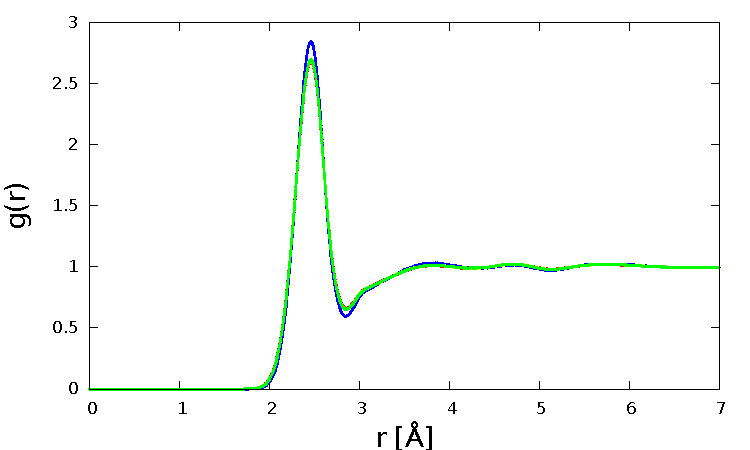
\includegraphics[width=0.475\textwidth]
{figures/fixedpoint.pdf}
\end{center}
\caption{\label{Fig1}
Partial pair correlation function for liquid Si at 3000~K with noisy forces introduced by fixed-point errors of magnitude $10^{-3}$ (green), $10^{-2}$ (yellow) and $10^{-1}$ (blue). For comparison, the results, as obtained by our reference calculations without noise, are shown in red. 
} \end{figure}
In Figs.~\ref{Fig1} and \ref{Fig2}, the Si-Si partial pair-correlation function $g(r)$, as computed using an optimal scheme for orthorombic systems \cite{KAF}, is shown for different values of $\beta$. %In Fig. 1 we show the pair correlation functions g(r) calculated with noisy forces generated from fixed-point errors. In Fig. 2 we show the pair correlation functions g(r) calculated with noisy forces generated with floating-point errors. 
As can be seen, for both fixed-point and floating-point errors, the agreement with our reference calculation is nearly perfect up to the highest noise we have investigated. As already anticipated earlier, the usage of floating-point errors is not only able to tolerate higher noise levels, but is also throughout more accurate. 
\begin{figure}%[h!]
\begin{center}
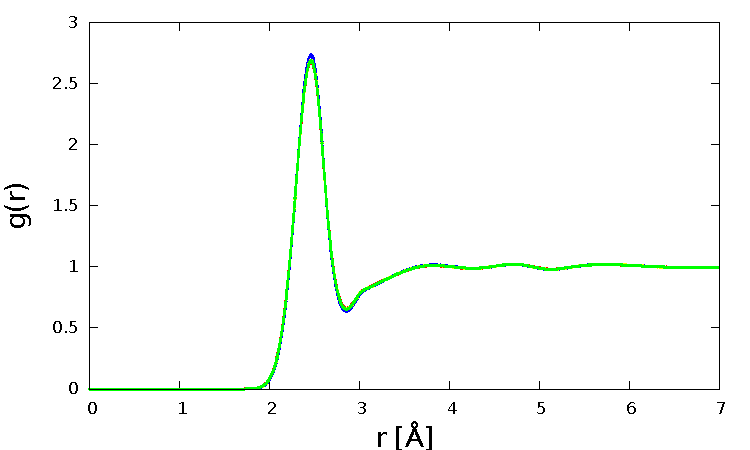
\includegraphics[width=0.475\textwidth]
{figures/floatingpoint.pdf}
\end{center}
\caption{\label{Fig2}
Partial pair correlation function for liquid Si at 3000~K with noisy forces introduced by floating-point errors of magnitude $10^{-2}$ (green), $10^{-1}$ (yellow) and $10^{-0}$ (blue). For comparison, the results, as obtained by our reference calculations without noise, are shown in red. 
} \end{figure}

To verify that the sampling is indeed canonical, in Fig.~\ref{Fig3} the actual kinetic energy distribution as obtained by our simulations using noisy forces and compared to the analytic Maxwell distribution. It is evident that if sampled long enough, not only the mean value, but also the the distribution tails are in excellent agreement with the exact Maxwellian kinetic energy distribution.
\begin{figure}%[h!]
\begin{center} 
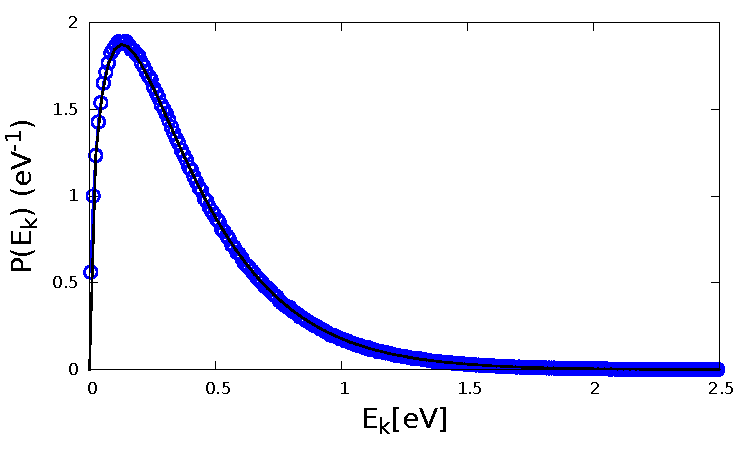
\includegraphics[width=0.475\textwidth]
{figures/maxwelldistribution.pdf}
\end{center}
\caption{\label{Fig3}
Kinetic energy distribution of liquid Si at 3000~K, as obtained by our simulations using noisy forces (blue circles). For comparison the amalytic Maxwell distribution is also shown (red line).
} \end{figure}
To further assess the accuracy of the present method, we expand the autocorrelation of the noisy forces, i.e. 
%\begin{equation}
%\begin{split}
%\left \langle \textbf{F}_{I}^{N}\left ( 0 \right )\textbf{F}_{I}^{N}\left ( t \right )\right \rangle = \linebreak \\ \left \langle \left ( \textbf{F}_{I}\left ( 0 \right ) + \mathbf{\Xi } _{I}^{N}\left(0 \right )\right) \left( \textbf{F}_{I}\left ( t \right )+\mathbf{\Xi } _{I}^{N}\left ( t \right )\right) \right \rangle
%\end{split}
%\end{equation}
\begin{subequations}
\begin{eqnarray}
  && \left \langle \textbf{F}_{I}^{N}\left ( 0 \right )\textbf{F}_{I}^{N}\left ( t \right )\right \rangle \\
  &=& \left \langle \left ( \textbf{F}_{I}\left ( 0 \right ) + \mathbf{\Xi } _{I}^{N} \left(0 \right )\right) \left( \textbf{F}_{I}\left ( t \right )+\mathbf{\Xi } _{I}^{N}\left ( t \right )\right) \right \rangle \\
  &=& \left \langle \textbf{F}_{I}\left ( 0 \right ) \textbf{F}_{I}\left ( t \right )\right \rangle + \left \langle \textbf{F}_{I}\left ( 0 \right ) \mathbf{\Xi } _{I}^{N}\left(t \right )\right \rangle \label{AutoCorr} \\ 
  &+& \left \langle \textbf{F}_{I}\left ( t \right ) \mathbf{\Xi } _{I}^{N}\left(0 \right )\right \rangle + \left \langle \mathbf{\Xi } _{I}^{N}\left(0 \right ) \mathbf{\Xi } _{I}^{N}\left(t \right )\right \rangle.  \nonumber
\end{eqnarray}
\end{subequations}
%\begin{equation}\label{eq:1}
%\begin{split}
%\left \langle \textbf{F}_{I}^{N}\left ( 0 \right )\textbf{F}_{I}^{N}\left ( t \right )\right \rangle = \left \langle \textbf{F}_{I}\left ( 0 \right ) \textbf{F}_{I}\left ( t \right )\right \rangle + \linebreak \\\left \langle \textbf{F}_{I}\left ( 0 \right ) \mathbf{\Xi } _{I}^{N}\left(t \right )\right \rangle +  \left \langle \textbf{F}_{I}\left ( t \right ) \mathbf{\Xi } _{I}^{N}\left(0 \right )\right \rangle + \left \langle \mathbf{\Xi } _{I}^{N}\left(0 \right ) \mathbf{\Xi } _{I}^{N}\left(t \right )\right \rangle
%\end{split}
%\end{equation}
Since the cross correlation terms between the exact force and the additive white noise is vanishing due to Eq.~\ref{CrossCorr}, comparing the autocorrelation of the noisy forces $\langle \textbf{F}_{I}^{N}(0)\textbf{F}_{I}^{N}(t)\rangle$ with the autocorrelation of the exact forces $\langle \textbf{F}_{I}(0) \textbf{F}_{I}(t)\rangle$ permits to assess the localization of the last term of Eq.~\ref{AutoCorr}.
%Since, due to fluctuation-dissipation theorem, the last term of Eq.~\ref{AutoCorr} corresponds to a $\delta$-function, comparing the autocorrelation of the noisy forces $\langle \textbf{F}_{I}^{N}(0)\textbf{F}_{I}^{N}(t)\rangle$ with the autocorrelation of the exact forces $\langle \textbf{F}_{I}(0) \textbf{F}_{I}(t)\rangle$ permits to assess the cross correlation terms between the exact force and the additive white noise. 
The fact that $\langle \textbf{F}_{I}^{N}(0)\textbf{F}_{I}^{N}(t)\rangle$ is essentially identical to $\langle \textbf{F}_{I}(0) \textbf{F}_{I}(t)\rangle$, as can be seen in Fig.~\ref{Fig4}, implies that $\langle \mathbf{\Xi } _{I}^{N}(0) \mathbf{\Xi } _{I}^{N}(t)\rangle$ is very close to a $\delta$-function as required by the fluctuation-dissipation theorem in order to ensure an accurate canonical sampling of the Boltzmann distribution. 
\begin{figure}%[h!]
\begin{center}
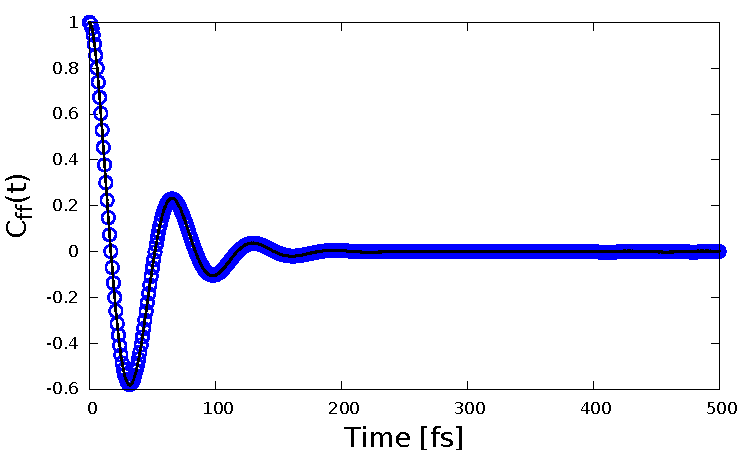
\includegraphics[width=0.475\textwidth]
{figures/force_autocorrelation.pdf}
\end{center}
\caption{\label{Fig4}
The Autocorrelation of the noisy forces \(
\left \langle \textbf{F}_{I}^{N}\left ( 0 \right ) \textbf{F}_{I}^{N}\left ( t \right )\right \rangle \)(line), which are compared to the autocorrelation of the exact forces \( \left \langle \textbf{F}_{I}\left ( 0 \right ) \textbf{F}_{I}\left ( t \right )\right \rangle \)(circles). 
} \end{figure}

%If the random value that was used to generate the computational error is chosen in the range [0,1] instead of [-0.5,0.5], we encounter a phenomenon called "Flying Ice Cube" \cite{flyingIceCube} during our MD simulations.  


\section{Summary}
To summarize, in this paper, we described the method to compensate for the computational errors that are introduced when running the MD code in FPGA or GPU using approximate computing technique.  



\begin{acknowledgments}
The authors would like to thank the Gauss Center for Supercomputing (GCS) for providing computing time through the John von Neumann Institute for Computing (NIC) on the GCS share of the supercomputer JUQUEEN at the J\"ulich Supercomputing Centre (JSC). This project has received funding from the European Research Council (ERC) under the European Union's Horizon 2020 research and innovation programme (grant agreement No 716142).
\end{acknowledgments}


\bibliography{report}


\end{document}
